\documentclass[tikz, border=5pt]{standalone}

\usepackage{amsmath,amssymb}
\usepackage{xcolor}
\usetikzlibrary{arrows.meta, shadows.blur, shapes.geometric, calc}

\definecolor{utnblue}{RGB}{0, 51, 102}

\begin{document}
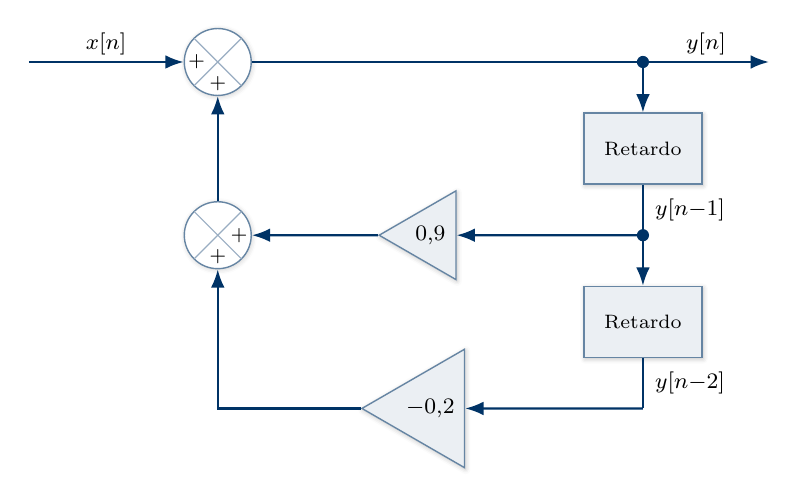
\begin{tikzpicture}[>=Latex, font=\small,
    gain_l/.style={
        regular polygon, regular polygon sides=3, shape border rotate=210,
        draw=utnblue!60, line width=0.5pt, fill=utnblue!8,
        minimum size=1.3cm, inner sep=0pt, font=\footnotesize,
        blur shadow={shadow blur steps=4, shadow blur extra rounding=0pt,
                     shadow xshift=0.4pt, shadow yshift=-0.6pt, shadow opacity=25}
    },
    delay/.style={
        draw=utnblue!60, line width=0.5pt, fill=utnblue!8,
        minimum width=1.5cm, minimum height=0.9cm, font=\scriptsize,
        blur shadow={shadow blur steps=4, shadow blur extra rounding=0pt,
                     shadow xshift=0.4pt, shadow yshift=-0.6pt, shadow opacity=25}
    },
    sum/.style={
        draw=utnblue!60, line width=0.5pt, circle, minimum size=0.85cm,
        inner sep=0pt, fill=white,
        blur shadow={shadow blur steps=4, shadow blur extra rounding=0pt,
                     shadow xshift=0.3pt, shadow yshift=-0.4pt, shadow opacity=20}
    },
    cross_line/.style={utnblue!40, line width=0.4pt},
    signal/.style={->, thick, utnblue},
    wire/.style={-, thick, utnblue},
    tlab/.style={font=\footnotesize, inner sep=2pt, text=black},
]

\newcommand{\sumcross}[1]{%
    \draw[cross_line] ($(#1)+(-0.30,-0.30)$) -- ($(#1)+(0.30,0.30)$);
    \draw[cross_line] ($(#1)+(-0.30,0.30)$) -- ($(#1)+(0.30,-0.30)$);
}

    % --- columna central de sumadores ---
    \node[sum] (S0) at (0,0) {};
    \sumcross{S0}
    \node[font=\scriptsize] at ($(S0)+(-0.27,0)$) {$+$};
    \node[font=\scriptsize] at ($(S0)+(0,-0.27)$) {$+$};

    \node[sum] (S1) at (0,-2.2) {};
    \sumcross{S1}
    \node[font=\scriptsize] at ($(S1)+(0.27,0)$) {$+$};
    \node[font=\scriptsize] at ($(S1)+(0,-0.27)$) {$+$};

    % --- escaladores y retardos ---
    \node[gain_l] (g1) at (2.7,-2.2) {$0{,}9$};
    \node[gain_l] (g2) at (2.7,-4.4) {$-0{,}2$};
    \node[delay]  (D1) at (5.4,-1.1) {Retardo};
    \node[delay]  (D2) at (5.4,-3.3) {Retardo};

    % --- espinas de entrada y salida ---
    \coordinate (in)    at (-2.4,0);
    \coordinate (otap)  at (5.4,0);
    \coordinate (out)   at (7.0,0);
    \coordinate (tone)  at (5.4,-2.2);
    \coordinate (ttwo)  at (5.4,-4.4);

    \draw[signal] (in) -- (S0.west) node[tlab, above, midway] {$x[n]$};
    \draw[wire]   (S0.east) -- (otap);
    \fill[utnblue] (otap) circle (2.2pt);
    \draw[signal] (otap) -- (out) node[tlab, above, midway] {$y[n]$};
    \draw[signal] (otap) -- (D1.north);

    % --- cadena de retardos y realimentaciones ---
    \draw[wire]   (D1.south) -- (tone)
                  node[tlab, midway, anchor=west, xshift=2pt] {$y[n{-}1]$};
    \fill[utnblue] (tone) circle (2.2pt);
    \draw[signal] (tone) -- (g1.east);
    \draw[signal] (tone) -- (D2.north);

    \draw[wire]   (D2.south) -- (ttwo)
                  node[tlab, midway, anchor=west, xshift=2pt] {$y[n{-}2]$};
    \draw[signal] (ttwo) -- (g2.east);

    \draw[signal] (g1.west) -- (S1.east);
    \draw[signal] (g2.west) -| (S1.south);
    \draw[signal] (S1.north) -- (S0.south);

\end{tikzpicture}
\end{document}
